% Polished Appendix C: Additional Evaluation Material (proofread by Claude). Original text is in main-original.tex.
\section{Technical Appendix: Additional Evaluation Material}
\label{app:eval}

\paragraph{Matched evaluation.}
The 525 matched prompts combine 265 previously delivered BrickForma Q8\_0 exports with 260 supplemental exports. We score the single raw export supplied for each prompt. This protocol measures the delivered drafts as they are: it does not filter on completion or geometry, rerun Algorithm~\ref{alg:inference-refinement}, or choose candidates by score. The supplemental records flag 8 incomplete generations and 96 failures of the source geometry check among the 260 exports; the two sets may overlap. The 265 earlier exports have no corresponding completion or geometry flags. We score all 1,575 LDraw exports on all four metrics, using 12,600 rendered views for alignment. Because three supplied GLB previews contain only a prefix of the assembly, we render from the delivered LDraw sequences in all cases. BrickGPT uses a $20^3$ world and seed 42, with recorded regeneration budgets of 8 or 100. The 260 supplemental BrickForma exports were generated locally without MILP refinement, using checkpoint \texttt{BrickGPT-Qwen3-1.7B-BrickMore-48} (revision \texttt{92d1c595}) in \texttt{bfloat16} precision with \texttt{sdpa} attention, \texttt{max\_new\_tokens}=8192, \texttt{temperature}=0.7, \texttt{top\_p}=0.9, and the seed schedule $(42,104,2026)$, with zero overlap with the training set. The 265 earlier Q8\_0 exports come from an earlier inference batch whose per-sample decoding flags were not logged. Finally, the 105-sample difference between $79{,}301{\times}5=396{,}505$ and the 396,610 logged training pairs stems from a minor snapshot offset between the final dataset release and the training run.

\begin{samepage}
\paragraph{Baseline versions.} The archived 260-prompt BrickGPT runner is based on GitHub commit \texttt{9c53c7c} of \url{https://github.com/AvaLovelace1/BrickGPT}. Its generation report records a local checkpoint that combines \texttt{meta-llama/Llama-3.2-1B-Instruct} with the public \texttt{AvaLovelace/BrickGPT} LoRA adapter. The runner can load a premerged checkpoint or merge these weights through PEFT's \texttt{merge\_and\_unload}; the report identifies the merged checkpoint used, but no separate merge log exists. The BrickNet GitHub reference snapshot is commit \texttt{283faf7} of \url{https://github.com/kulits/BrickNet}, and the public 1.7B PT and SFT adapter revisions on \texttt{Qwen/Qwen3-1.7B} are \texttt{0f75d5e5} and \texttt{3fe7f4c1}, respectively. The other 265 BrickGPT exports and the BrickNet exports have no recorded generation-code commit. Invalid-placement scoring uses the inset collision kernel from the pinned \texttt{bricknet==0.1.0} PyPI wheel.

\paragraph{Reference dataset snapshots.} BrickGPT uses StableText2Brick (public data upload \texttt{1dcf904} at \texttt{AvaLovelace/StableText2Brick}). BrickNet uses the gated PT, SFT, and validation splits described in \texttt{DATA.md} at GitHub commit \texttt{283faf7}; the release documentation identifies these splits by file name and gives no separate dataset revision.
\end{samepage}

\paragraph{Untuned Qwen3-1.7B.} None of the 260 untuned outputs passed the generation-time geometry check. The strict parser found no placements in 178 outputs, and two more used an unsupported part type. We assign these 180 outputs zero VQAScore, PE, and SigLIP2, and keep the measured scores for the 80 scorable partial layouts, so all alignment means are over the same 260 prompts. On the 80 pairs with scorable base layouts, the mean file-order invalid-placement ratio is 39.67\% for the untuned model and 1.01\% for raw BrickForma. The comparison applies common scoring to delivered generation runs whose decoding settings may differ.

\paragraph{Paired tests and truncation.}
Table~\ref{tab:sig} compares alignment scores on the 525 prompts. We use a two-sided exact sign test and a two-sided Wilcoxon signed-rank test with the normal approximation, excluding ties, and apply Holm correction separately to the six comparisons within each test. All adjusted $p$ values are below $2.0{\times}10^{-8}$. PE truncates 121 prompts and SigLIP2 truncates 209. On the untruncated subsets, BrickForma, BrickGPT, and BrickNet score 0.1510, 0.1408, and 0.1135 on PE (404 prompts) and 0.0340, 0.0157, and 0.0009 on SigLIP2 (316 prompts).

\begin{table}[t]
\centering\small
\setlength{\tabcolsep}{3pt}
\begin{tabular}{llrrr}
\toprule
Baseline & Metric & W/L/T & Sign $p_H$ & Wilc.\ $p_H$ \\
\midrule
BrickGPT & VQAScore & 384/141/0 & $1.5\times 10^{-26}$ & $4.8\times 10^{-20}$ \\
 & PE & 337/188/0 & $1.6\times 10^{-10}$ & $3.1\times 10^{-12}$ \\
 & SigLIP2 & 327/198/0 & $2.0\times 10^{-8}$ & $7.3\times 10^{-12}$ \\
BrickNet & VQAScore & 460/65/0 & $1.6\times 10^{-73}$ & $4.6\times 10^{-60}$ \\
 & PE & 406/119/0 & $4.6\times 10^{-37}$ & $1.3\times 10^{-47}$ \\
 & SigLIP2 & 408/115/2 & $9.4\times 10^{-39}$ & $2.4\times 10^{-42}$ \\
\bottomrule
\end{tabular}
\caption{Two-sided paired tests on the 525 prompts. W/L/T counts BrickForma's wins, losses, and ties. Each test applies Holm correction across its six comparisons.}
\label{tab:sig}
\end{table}


\paragraph{Earlier 114-prompt comparison.} BrickGPT outputs were generated in its native $20^3$ world (seed 42), whereas BrickForma places bricks in a $48^3$ workspace, which partly explains the difference in part counts. The systems also differ in candidate selection, filtering, and post-processing. On the BrickForma side, 45 of the 114 comparison outputs, together with their prompts, were chosen by human review as the best of six candidate phrasings in a category--level group; a winner was found in 79 of the 105 groups, and 45 of those winners entered this comparison. The remaining 69 outputs come from later fill-in, regeneration, collaborator, and review rounds: 35 replaced a judged winner in 34 groups, and 34 filled 26 groups in which no candidate had been judged acceptable. Together, the 114 outputs cover all 105 groups.\footnote{The six candidates are the five new-batch phrasings and one first-batch phrasing documented in the evaluation-set README. Of the 69 later outputs, 21 come from a review round, 16 and 7 from two collaborator-contributed sets, 12 from a second-round redo, 7 from a third-round fill-in, 5 from regeneration, and 1 from a car-specific trial, as recorded in the delivery manifest. BrickGPT was then run once on each selected prompt (seed 42), and BrickNet contributed one accepted sample per prompt (up to 30 attempts).} The 114 outputs comprise 110 refined layouts and four raw layouts. The earlier BrickGPT records report an eight-regeneration budget with Gurobi disabled.

\paragraph{Sensitivity of the earlier comparison.}
With equal weighting over the 105 category--level groups, BrickForma scores 0.2347, 0.1840, and 0.1257 and BrickGPT scores 0.1511, 0.1459, and 0.0318 on VQAScore, PE, and SigLIP2, respectively. After excluding prompts truncated by each encoder, PE is 0.1821 versus 0.1445 on 89 prompts, and SigLIP2 is 0.1088 versus 0.0301 on 85 prompts. The PE and SigLIP2 text encoders read at most 72 and 64 tokens, respectively.

\paragraph{Inference refinement.}
For the clipped voxel union $C$, let $\mathcal{B}(v)$ index the candidate placements from the oriented footprint library that cover $v$ and lie entirely within $C$. With binary placement variables $x_b$, exact coverage requires $\sum_{b\in\mathcal{B}(v)}x_b=1$ for each $v\in C$, which preserves the union and excludes overlaps. To enforce a single stud-connected component, a standard single-commodity flow formulation routes flow from a virtual root $r$ through directed stud-contact edges $(b,b')\in\mathcal{E}$ between adjacent layers. Grounded candidate placements $b\in\mathcal{B}_{\mathrm{gnd}}$ receive root inflow $f_{r,b}\ge 0$; internal edge flows satisfy $0\le f_{b,b'}\le M x_b$ and $0\le f_{b,b'}\le M x_{b'}$ with capacity bound $M=|C|$; and flow conservation $\sum_{(u,b)\in\mathcal{E}\cup\{(r,b)\}} f_{u,b} - \sum_{(b,v)\in\mathcal{E}} f_{b,v} = x_b$ ensures that every selected placement is connected to the root. We solve the MILP with SciPy's HiGHS interface under the time tiers of Algorithm~\ref{alg:inference-refinement}, and a feasible cover must also pass the independent placement, coverage, and connectivity audit. The logged run summaries record the solver time tiers and audit outcomes, but per-run objective weights and gap tolerances were not retained. Contact-based self-weight screening uses a separate LP (Appendix~\ref{app:dataset}).

\paragraph{Diagnostic cohort.}
To probe what the fine-tuned model learns, we inspected 525 BrickForma generations from a diagnostic set (21 categories $\times$ five levels $\times$ five phrasings). Together with 105 first-batch prompts, this diagnostic batch formed the six-phrasing candidate pool from which 45 of the 114 comparison outputs were selected (35 of them from the 525), as described above. Algorithm~\ref{alg:inference-refinement} describes the default candidate-selection and refinement rules. The diagnostic manifests record either a refinement tier or a raw layout kept unchanged. For 28 prompts, a recovery path sampled seeds outside $S$; for two further prompts, the solver budget was extended to 600\,s. Only 46 raw layouts (8.8\%) form a single stud-connected component without refinement. This rate shows no clear trend across levels (13, 9, 9, 7, and 8 for L1--L5) but varies strongly by category (e.g., 8/25 for sofa and 0/25 for basket and camera). All 479 failing raw layouts split into at least two stud components (median 5, maximum 33). Overlaps are a minor cause: 50 failing layouts contain duplicated voxels, 41 of them at most five (median 2), and 429 contain none. The 2,240 detached fragments are mostly airborne (1,320 airborne versus 920 grounded). The learned model thus places bricks whose in-bounds voxel union is retained by refinement but that often fail to interlock across layers; all 525 final assemblies form a single stud-connected component with that union unchanged (Table~\ref{tab:diag}). These checks evaluate stud connectivity and consistency of the in-bounds voxel union, not prompt-level shape fidelity or spatial reasoning.

\begin{figure*}[t]
\centering
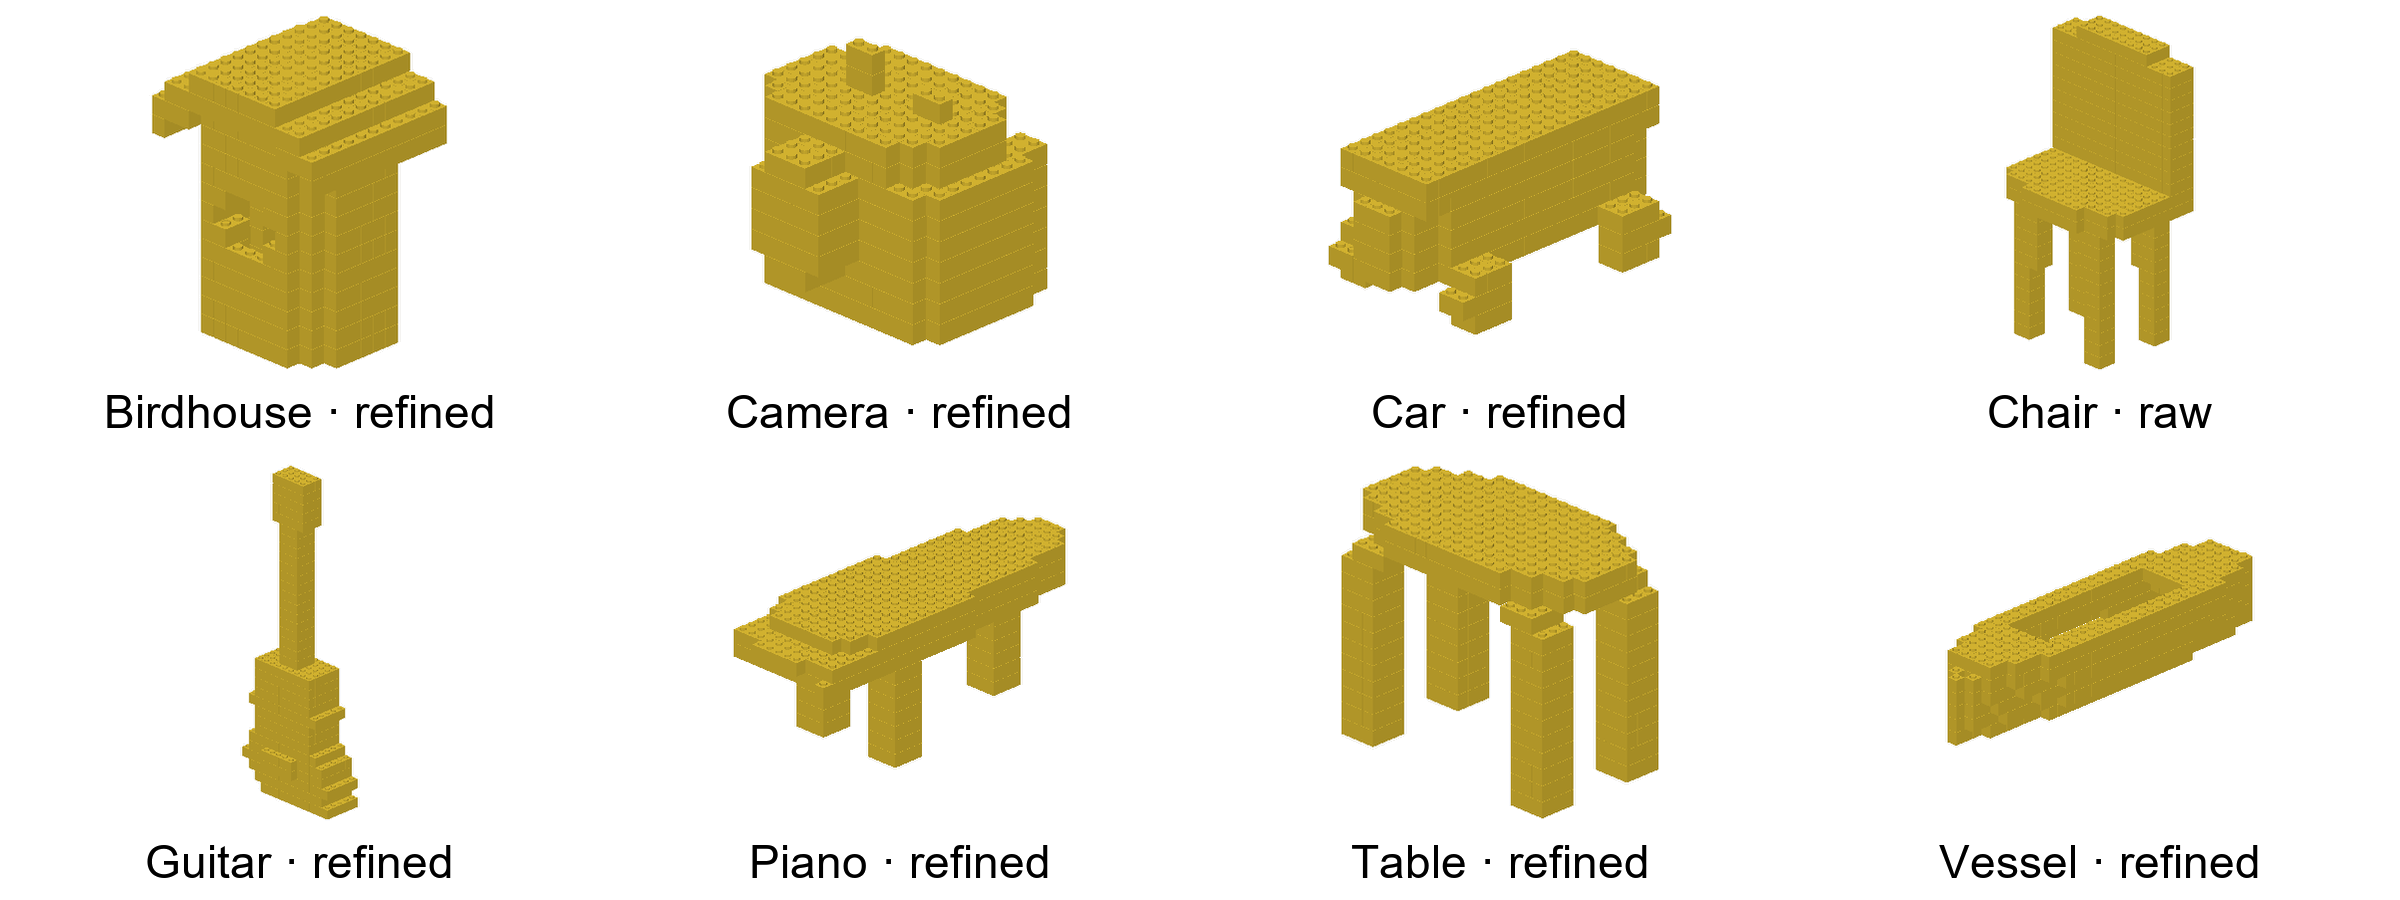
\includegraphics[width=\textwidth]{figures/generated_gallery_en.png}
\caption{BrickForma outputs from the earlier 114-prompt comparison. The chair is raw; the other examples are refined.}
\end{figure*}

\begin{table*}[!htbp]
\centering
\small
\setlength{\tabcolsep}{3pt}
\begin{tabular}{lr}
\toprule
Quantity (525 prompts) & Value \\
\midrule
Raw layout is a single stud component & 46 (8.8\%) \\
Stud components per failing raw layout (median / max) & 5 / 33 \\
Failing raw layouts with duplicated voxels & 50 / 479 \\
Detached fragments (airborne / grounded) & 1,320 / 920 \\
MILP tier reached (12 / 60 / 180 / 600\,s) & 326 / 133 / 18 / 2 \\
Prompts resampled outside $S$ & 28 \\
Final: single stud component, union unchanged & 525 / 525 \\
Raw bricks, median (range) & 183 (77--623) \\
Final assembly bricks, median & 452 \\
\bottomrule
\end{tabular}
\caption{Structural diagnostics of raw outputs (Section~\ref{sec:diagnostics}). ``Union unchanged'' means that the final assembly covers exactly the in-bounds voxel union of the raw draft; it does not assess whether the shape matches the prompt.}
\label{tab:diag}
\end{table*}

\begin{figure*}[!htbp]
\centering
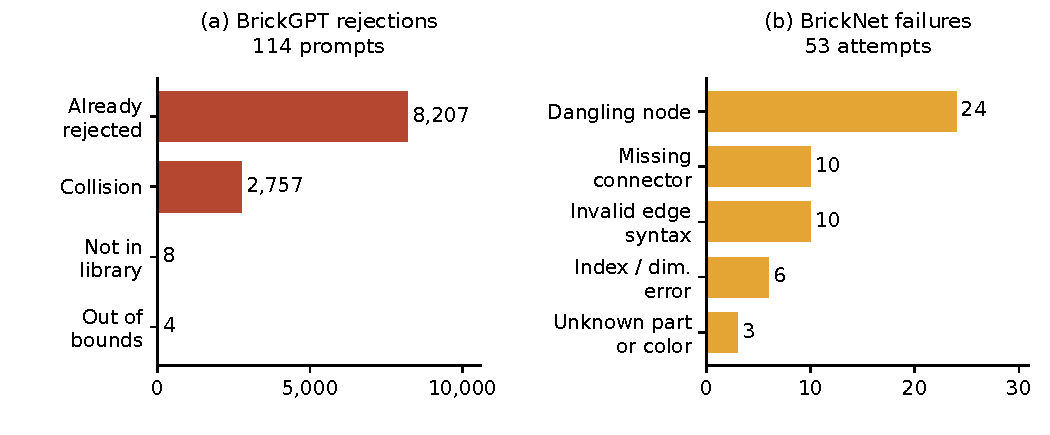
\includegraphics[width=\textwidth]{figures/image19_en.pdf}
\caption{Failure categories in the earlier 114-prompt comparison; values as given in the corresponding run records.}
\end{figure*}

\begin{figure*}[!htbp]
\centering
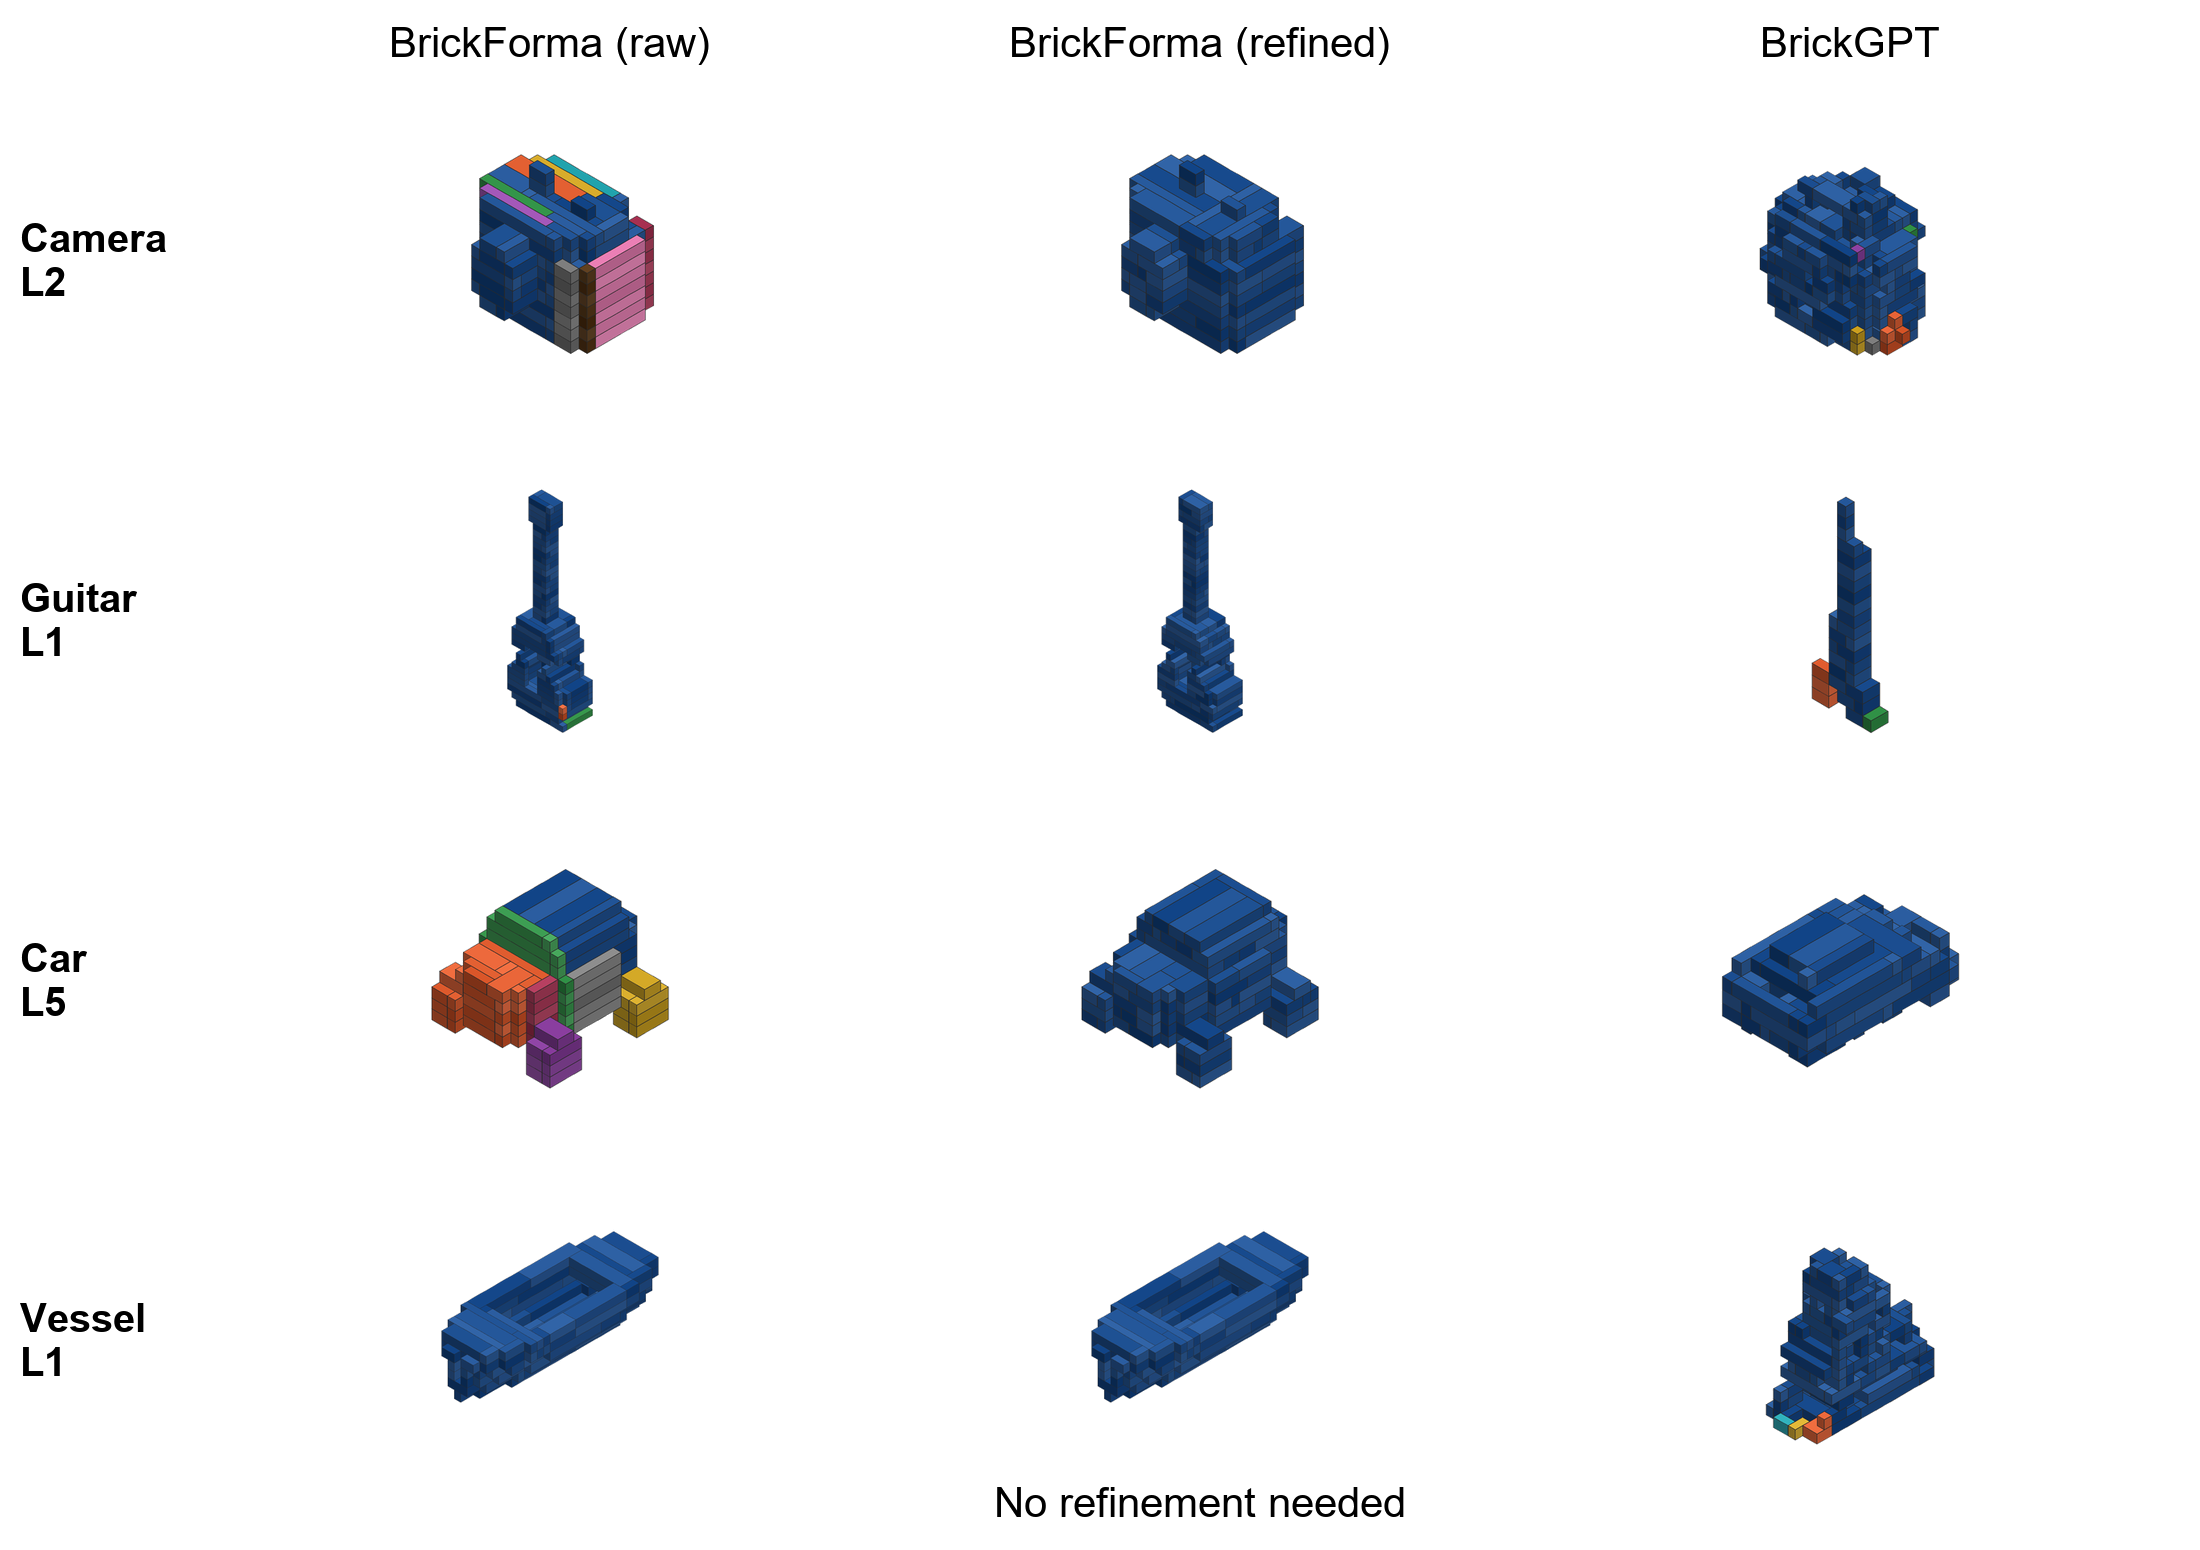
\includegraphics[width=\textwidth]{figures/original_comparison_en.png}
\caption{Qualitative examples from the earlier comparison. Columns show raw and refined BrickForma outputs and BrickGPT outputs.}
\end{figure*}

\begin{figure*}[t]
\centering
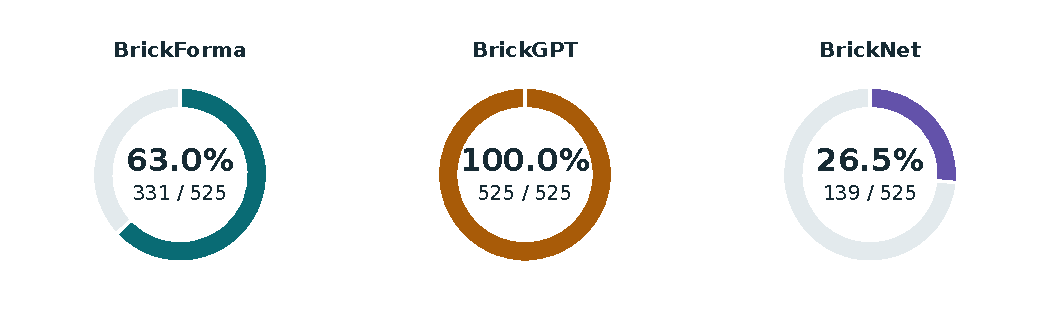
\includegraphics[width=\textwidth]{figures/comparison_20261117/01-zero-invalid.pdf}
\caption{Outputs with zero invalid placements on the 525 matched prompts. Colored arcs show outputs with $P_{\mathrm{inv}}=0$, and gray arcs show outputs with $P_{\mathrm{inv}}>0$. Each panel contains 525 outputs.}
\label{fig:comparison-zero-invalid}
\end{figure*}

\begin{figure*}[t]
\centering
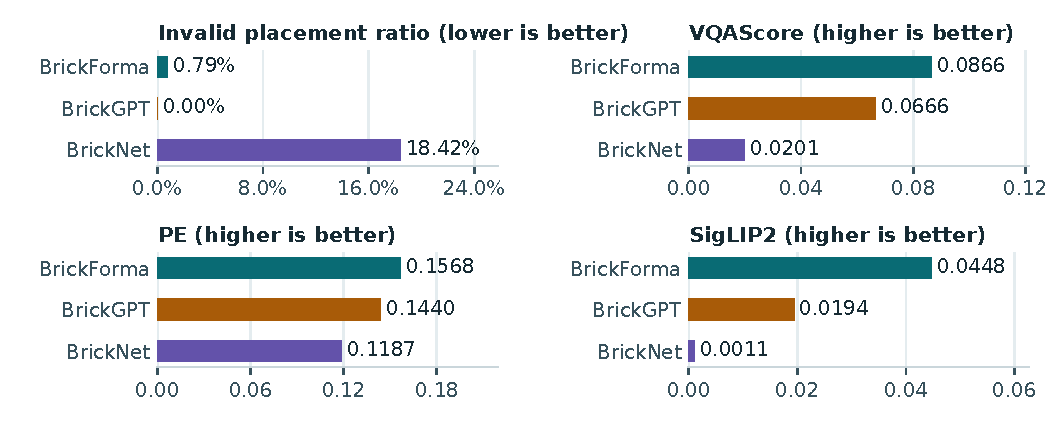
\includegraphics[width=\textwidth]{figures/comparison_20261117/02-means.pdf}
\caption{Mean scores on the 525 matched prompts. Each mean weights all prompts equally. The plotted values match Table~\ref{tab:main}.}
\label{fig:comparison-means}
\end{figure*}

\begin{figure*}[t]
\centering
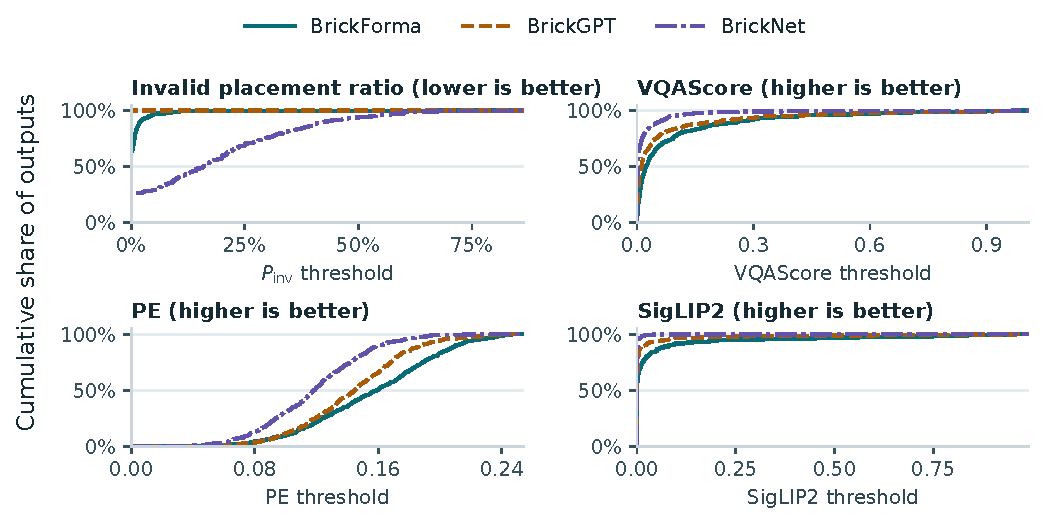
\includegraphics[width=\textwidth]{figures/comparison_20261117/03-distributions.pdf}
\caption{Empirical cumulative distributions of the four scores. Each curve gives the fraction of a system's 525 outputs that score at or below the threshold on the horizontal axis.}
\label{fig:comparison-distributions}
\end{figure*}

\begin{figure*}[t]
\centering
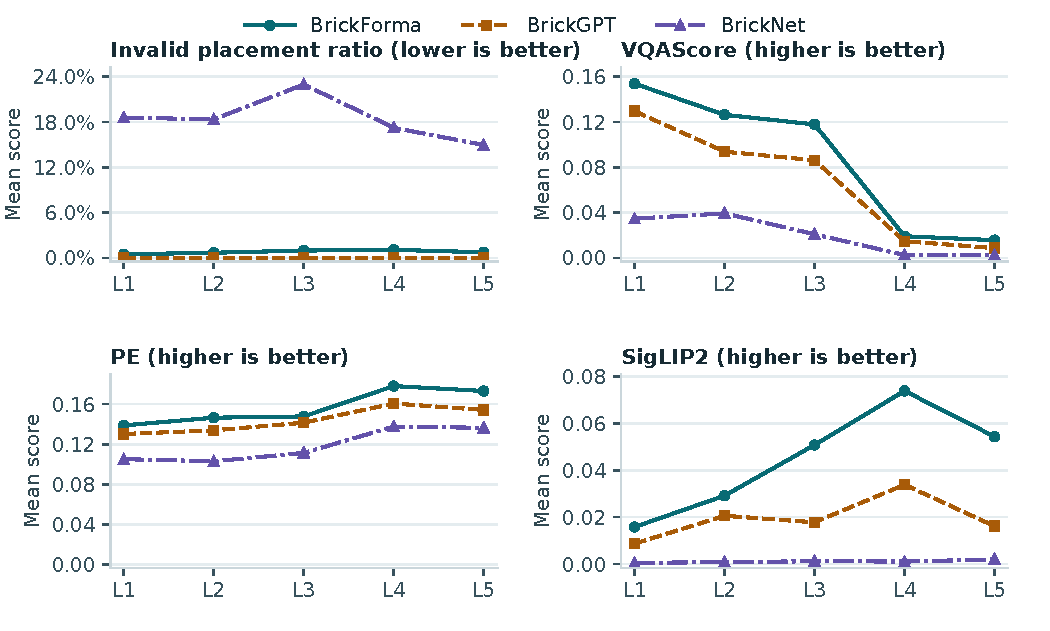
\includegraphics[width=\textwidth]{figures/comparison_20261117/04-by-level.pdf}
\caption{Mean scores from L1 to L5. Each point averages the 105 prompts shared by all three systems at that level (Table~\ref{tab:level-results}). From L3 to L4, VQAScore falls for all three systems, while PE rises.}
\label{fig:comparison-levels}
\end{figure*}

